\chapter{Progettazione concettuale e logica}
In questo capitolo verranno analizzati i requisiti che deve rispettare il database, e verr\`a quindi definito lo schema Entity-Relationship. Nel caso ci sia la necessit\`a
di definire dei vincoli non esprimibili tramite lo schema ER, verranno inoltre definiti dei vincoli esterni.
\section{Requisiti del database}
L'applicazione prevede la presenza di un Wallet associato a ciascun tenant, che pu\`o essere ricaricato tramite pagamenti effettuati con \textbf{Stripe}.
All'interno del sistema sono previsti dei \textbf{workflow}, processi che utilizzano dati provenienti da banche dati esterne per effettuare analisi di vario tipo.
Ogni operazione all'interno del workflow ha un costo, e per ognuna di queste viene scalato un determinato importo in base a un listino prezzi associato al tenant di appartenenza dell'utente.
Quando un'operazione viene inserita nella coda pagamenti, questa viene processata dal Credit Manager e registrata nel database, e il relativo importo viene scalato automaticamente dal Wallet del tenant.
Deve inoltre essere possibile annullare un'operazione. I listini sono sono costituiti da una descrizione e una fascia di prezzo, e specificano un importo per ogni tipo di operazione.

\section{Progettazione concettuale}
\subsection{Schema Entity-Relationship}
Uno schema ad alto livello: \`e uno schema orientato puramente alla definizione dei dati e delle relazioni tra loro, senza fare considerazioni su performance o altro.
Non sono presenti neanche le chiavi primarie normalmente richieste in un vero database.
\begin{figure}[H]
  \centering
  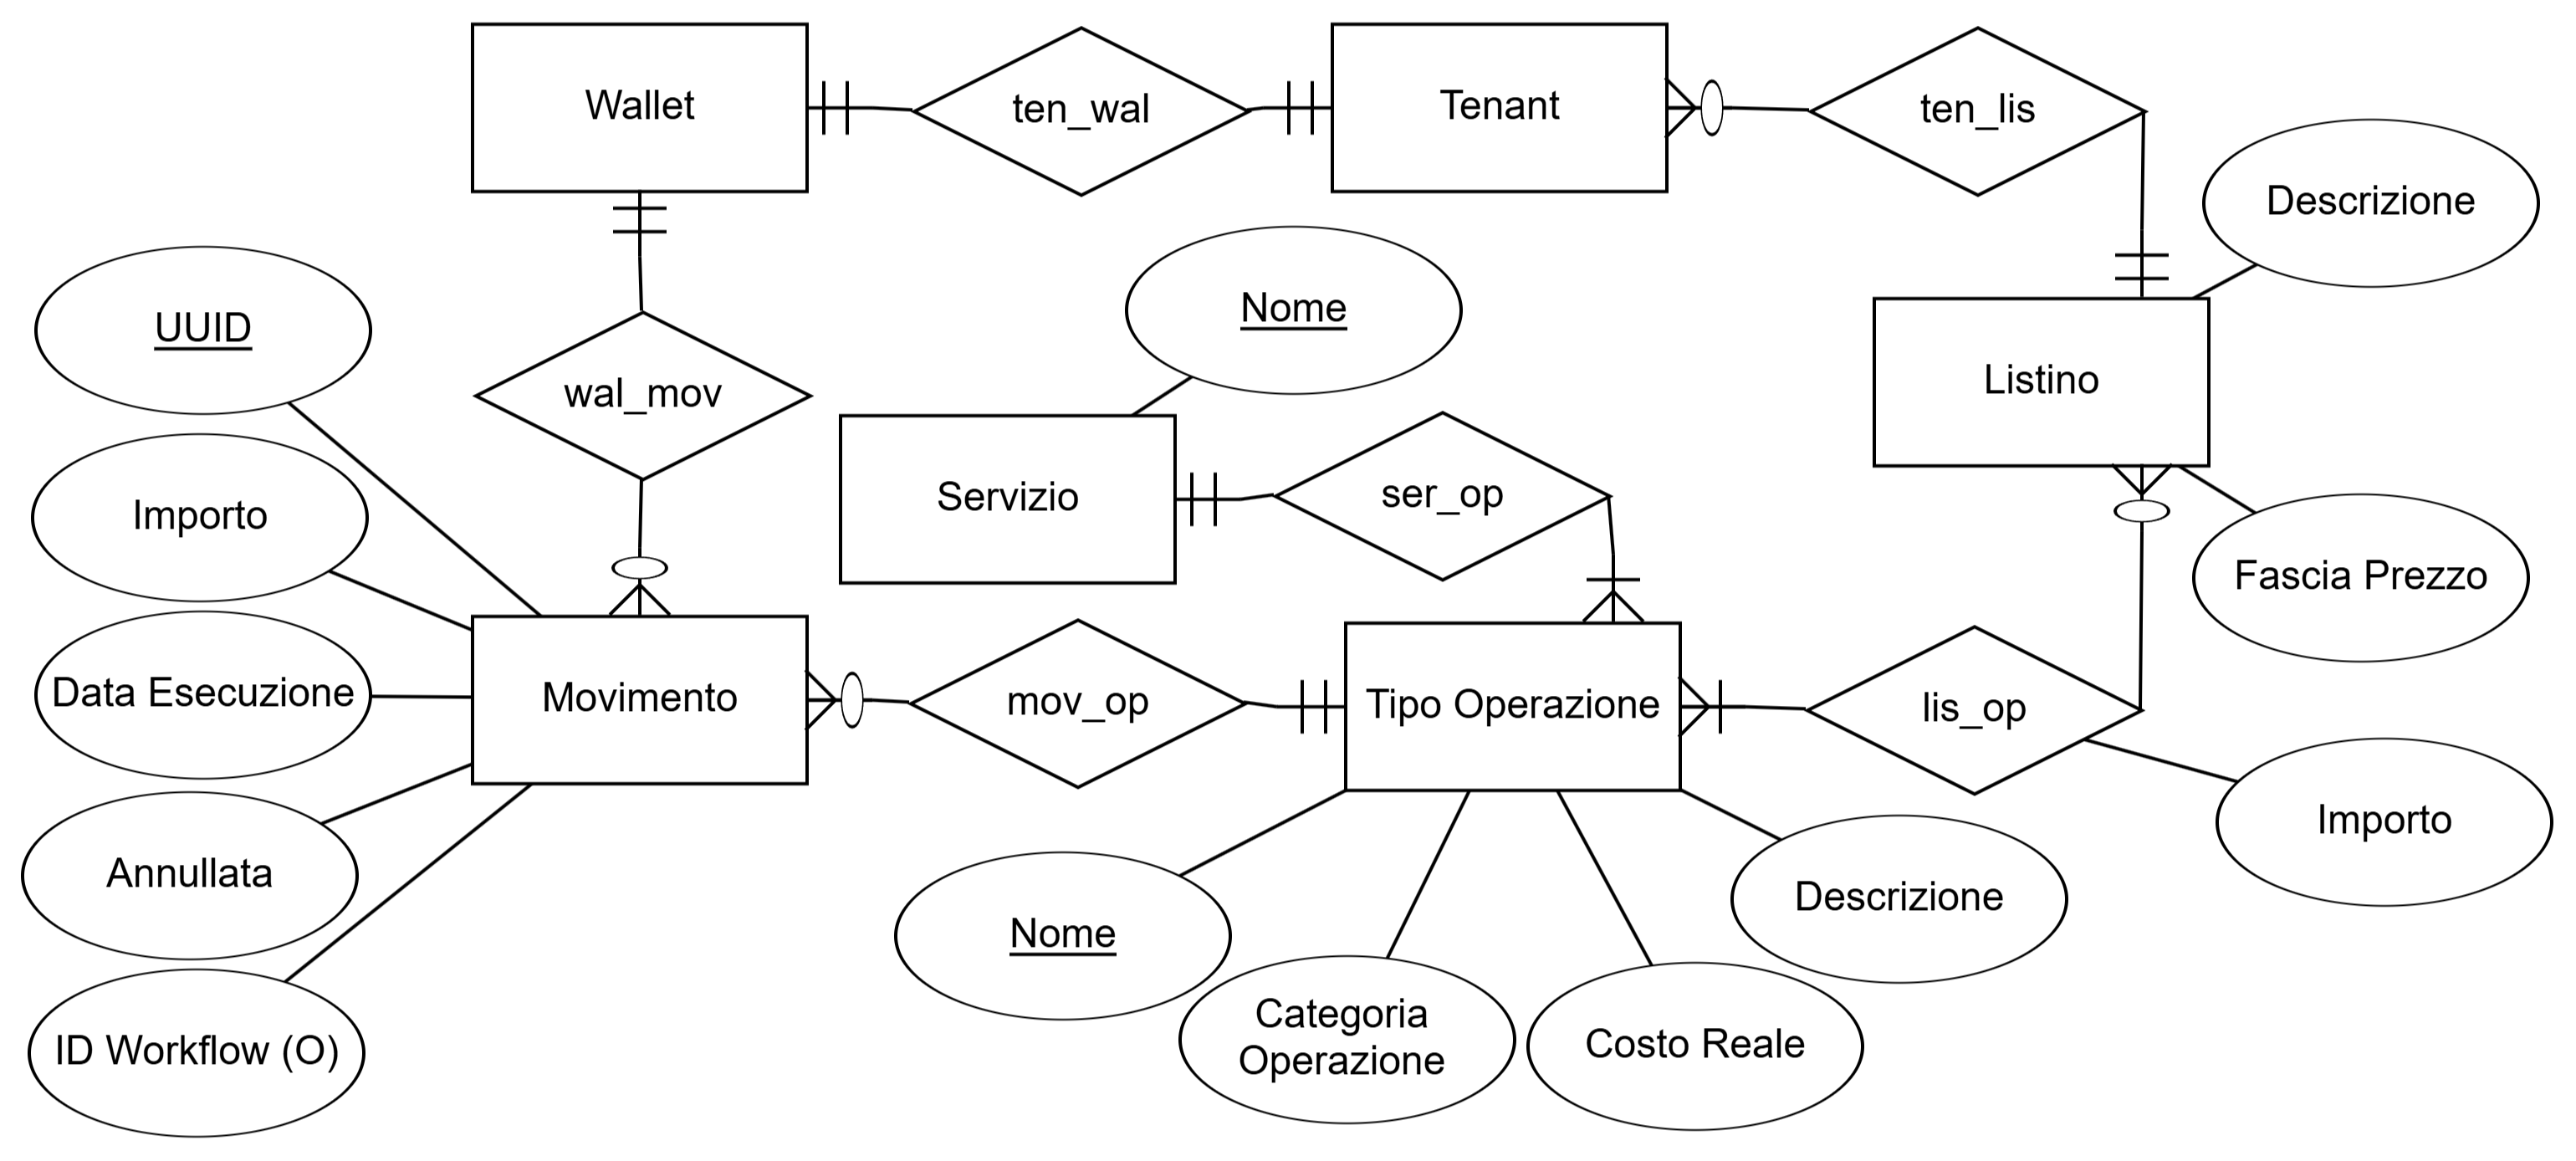
\includegraphics[width=12cm]{images/db-diagrams/er-diagram-concept.png}
  \caption{Schema Entity-Relationship del database}
\end{figure}

\begin{table}[H]
  \centering
  \caption{Descrizione degli attributi dell'entit\`a Movimento}
  \begin{tabulary}{0.9\textwidth}{p{3cm}p{2cm}L}
    \toprule
    \textbf{Attributo} & \textbf{Dominio} & \textbf{Descrizione} \\
    \midrule
    UUID & UUID & UUID dell'operazione all'interno del workflow \\\addlinespace
    Importo & Numeric & Importo pagato dall'utente \\\addlinespace
    Data Esecuzione & DataOra & Data e Ora di esecuzione del movimento \\\addlinespace
    ID Workflow & integer & Identificatore del Workflow di cui fa parte il movimento \\\addlinespace
    Annullata & booleana & Indica che l'operazione \`e stata annullata e ha un'operazione contraria che la bilancia \\\bottomrule
  \end{tabulary}
\end{table}

\begin{table}[H]
  \centering
  \caption{Descrizione degli attributi dell'entit\`a Servizio}
  \begin{tabulary}{\textwidth}{LLL}
    \toprule
    \textbf{Attributo} & \textbf{Dominio} & \textbf{Descrizione} \\
    \midrule
    Nome & string & Nome del Servizio \\\bottomrule
  \end{tabulary}
\end{table}

\begin{table}[H]
  \centering
  \caption{Descrizione degli attributi dell'entit\`a Tipo Movimento}
  \begin{tabulary}{0.9\textwidth}{p{2.3cm}p{2.7cm}L}
    \toprule
    \textbf{Attributo} & \textbf{Dominio} & \textbf{Descrizione} \\
    \midrule
    Nome & string & Nome del Tipo Operazione \\\addlinespace
    Categoria Operazione & \{ADDEBITO, ACCREDITO\} & Tipologia di operazione. Utilizziamo un enum type per rappresentare questo attributo. \\\addlinespace
    Costo Reale & numeric & Costo reale affrontato interrogando la banca dati esterna \\\addlinespace
    Descrizione & string & Breve descrizione di cosa fa l'operazione\\\bottomrule
  \end{tabulary}
\end{table}

\begin{table}[H]
  \centering
  \caption{Descrizione degli attributi della relationship Prezzo Listino}
  \begin{tabulary}{\textwidth}{p{2.3cm}p{2.3cm}L}
    \toprule
    \textbf{Attributo} & \textbf{Dominio} & \textbf{Descrizione} \\
    \midrule
    Importo & numeric & Importo che verr\`a scalato al tenant associato al listino prezzi\\\bottomrule
  \end{tabulary}
\end{table}

\subsection{Vincoli Esterni}
Non \`e stato possibile rappresentare un singolo vincolo attraverso lo schema ER:\\\\
\textbf{\label{tuttiimporticoncept}Tutti gli importi specificati} - Esiste una relationship Prezzo Listino tra ogni entit\`a Listino e ogni entit\`a Tipo Operazione

\section{Casi d'uso}
\begin{figure}[H]
  \centering
  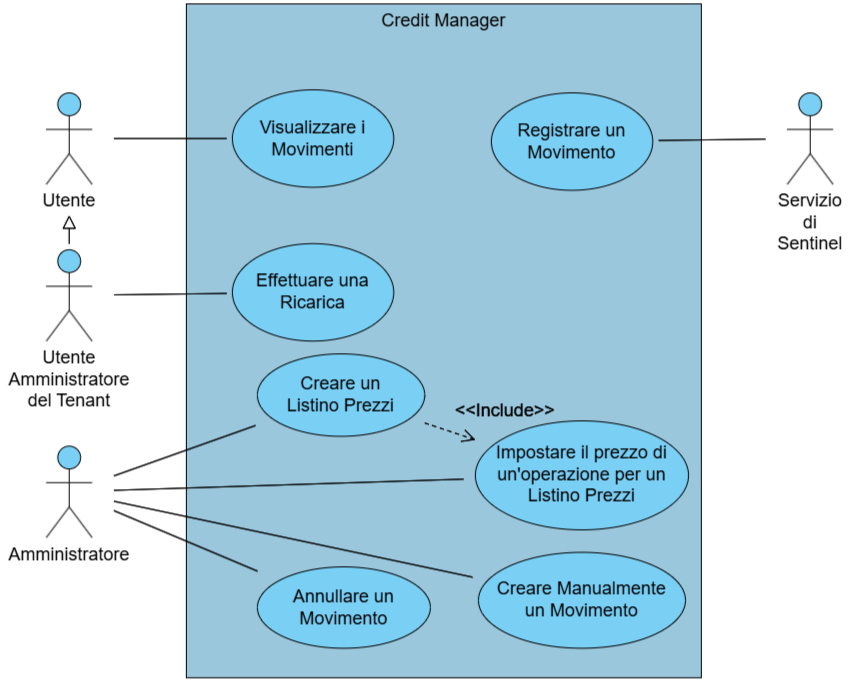
\includegraphics[width=10cm]{images/db-diagrams/use-case-diagram.jpg}
  \caption{Schema UML dei casi d'uso}
\end{figure}
